% MCP Semantic Annotations - Presentation Figures
% NOAA/EMC Environmental Information Branch
% December 18, 2025
%
% Compile with: pdflatex mcp_semantic_annotations_figures.tex
% Or use Overleaf for easy compilation

\documentclass[11pt]{article}
\usepackage[margin=1in]{geometry}
\usepackage{tikz}
\usetikzlibrary{shapes.geometric, arrows.meta, positioning, fit, backgrounds, calc}
\usepackage{xcolor}
\usepackage{pgfplots}
\pgfplotsset{compat=1.18}
\usepackage{booktabs}
\usepackage{float}
\usepackage{caption}
\usepackage{subcaption}

% NOAA-inspired color palette
\definecolor{noaablue}{RGB}{0, 84, 164}
\definecolor{noaadarkblue}{RGB}{0, 51, 102}
\definecolor{noaalightblue}{RGB}{135, 206, 235}
\definecolor{noaagreen}{RGB}{0, 128, 0}
\definecolor{noaaorange}{RGB}{255, 165, 0}
\definecolor{noaared}{RGB}{178, 34, 34}
\definecolor{noaagray}{RGB}{128, 128, 128}

% TikZ styles
\tikzstyle{component} = [rectangle, rounded corners, minimum width=3.5cm, minimum height=1cm, 
                         text centered, draw=noaablue, fill=noaalightblue!30, line width=1pt]
\tikzstyle{process} = [rectangle, minimum width=2.5cm, minimum height=0.8cm, 
                       text centered, draw=noaadarkblue, fill=noaablue!20]
\tikzstyle{data} = [cylinder, shape border rotate=90, draw=noaagreen, fill=noaagreen!20,
                    minimum height=1.2cm, minimum width=1.5cm]
\tikzstyle{arrow} = [-{Stealth[length=3mm]}, thick, noaablue]
\tikzstyle{dashedarrow} = [-{Stealth[length=3mm]}, thick, noaagray, dashed]

\title{\textbf{MCP Semantic Annotations for EE2 Compliance}\\
       \large Presentation Figures and Charts}
\author{NOAA/EMC Environmental Information Branch (EIB)}
\date{December 18, 2025}

\begin{document}

\maketitle
\tableofcontents
\newpage

%=============================================================================
\section{Architecture Overview}
%=============================================================================

\begin{figure}[H]
\centering
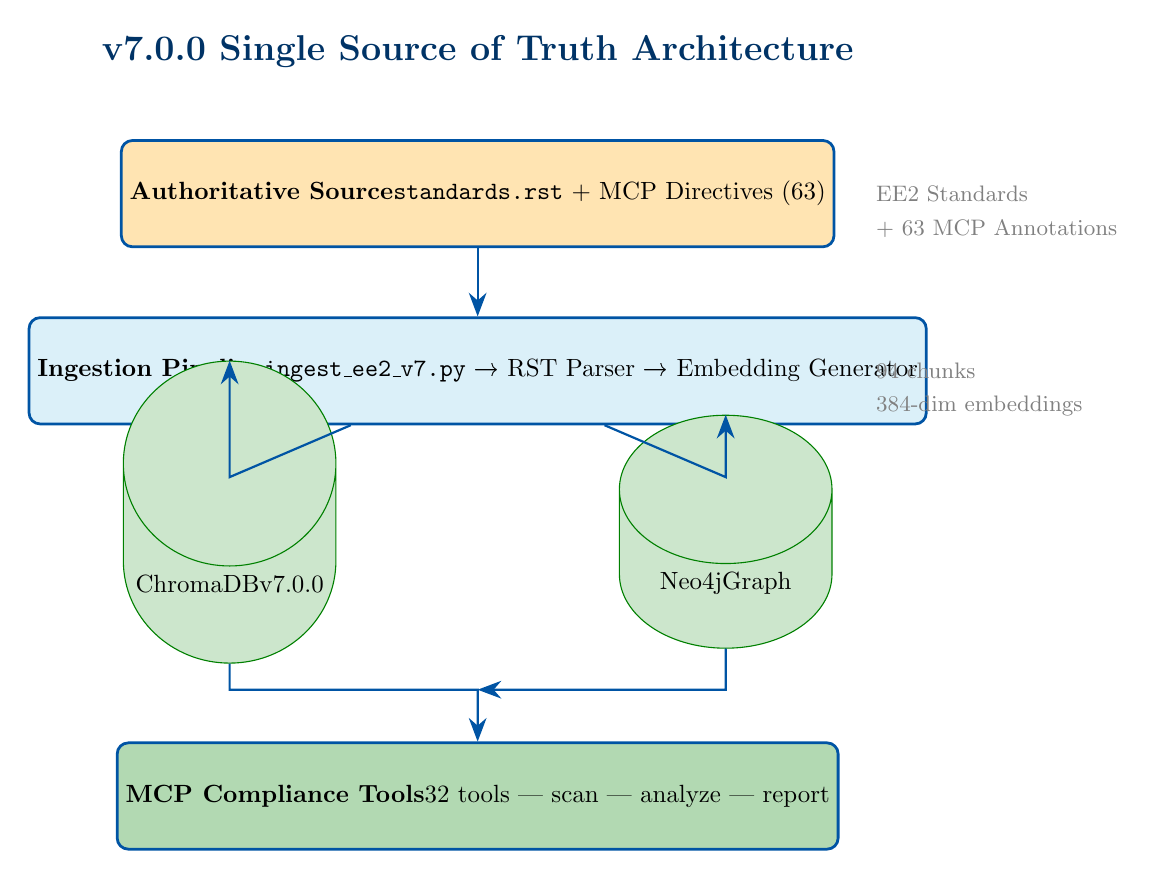
\begin{tikzpicture}[node distance=1.8cm, scale=0.9, transform shape]

% Title
\node[font=\Large\bfseries, noaadarkblue] at (0, 6) {v7.0.0 Single Source of Truth Architecture};

% Components
\node[component, minimum width=10cm, minimum height=1.5cm, fill=noaaorange!30] (source) at (0, 4) {
    \textbf{Authoritative Source}\\
    \texttt{standards.rst} + MCP Directives (63)
};

\node[component, minimum width=10cm, minimum height=1.5cm] (ingest) at (0, 1.5) {
    \textbf{Ingestion Pipeline}\\
    \texttt{ingest\_ee2\_v7.py} → RST Parser → Embedding Generator
};

\node[data, minimum width=3cm] (chromadb) at (-3.5, -1.5) {ChromaDB\\v7.0.0};
\node[data, minimum width=3cm] (neo4j) at (3.5, -1.5) {Neo4j\\Graph};

\node[component, minimum width=10cm, minimum height=1.5cm, fill=noaagreen!30] (tools) at (0, -4.5) {
    \textbf{MCP Compliance Tools}\\
    32 tools | scan | analyze | report
};

% Arrows
\draw[arrow] (source) -- (ingest);
\draw[arrow] (ingest) -- (-3.5, 0) -- (chromadb);
\draw[arrow] (ingest) -- (3.5, 0) -- (neo4j);
\draw[arrow] (chromadb) -- (-3.5, -3) -- (0, -3) -- (tools);
\draw[arrow] (neo4j) -- (3.5, -3) -- (0, -3);

% Annotations
\node[font=\small, noaagray, right] at (5.5, 4) {EE2 Standards};
\node[font=\small, noaagray, right] at (5.5, 3.5) {+ 63 MCP Annotations};
\node[font=\small, noaagray, right] at (5.5, 1.5) {94 chunks};
\node[font=\small, noaagray, right] at (5.5, 1) {384-dim embeddings};

\end{tikzpicture}
\caption{MCP Semantic Annotation Architecture (v7.0.0)}
\label{fig:architecture}
\end{figure}

\newpage
%=============================================================================
\section{Embedding Pipeline Flow}
%=============================================================================

\begin{figure}[H]
\centering
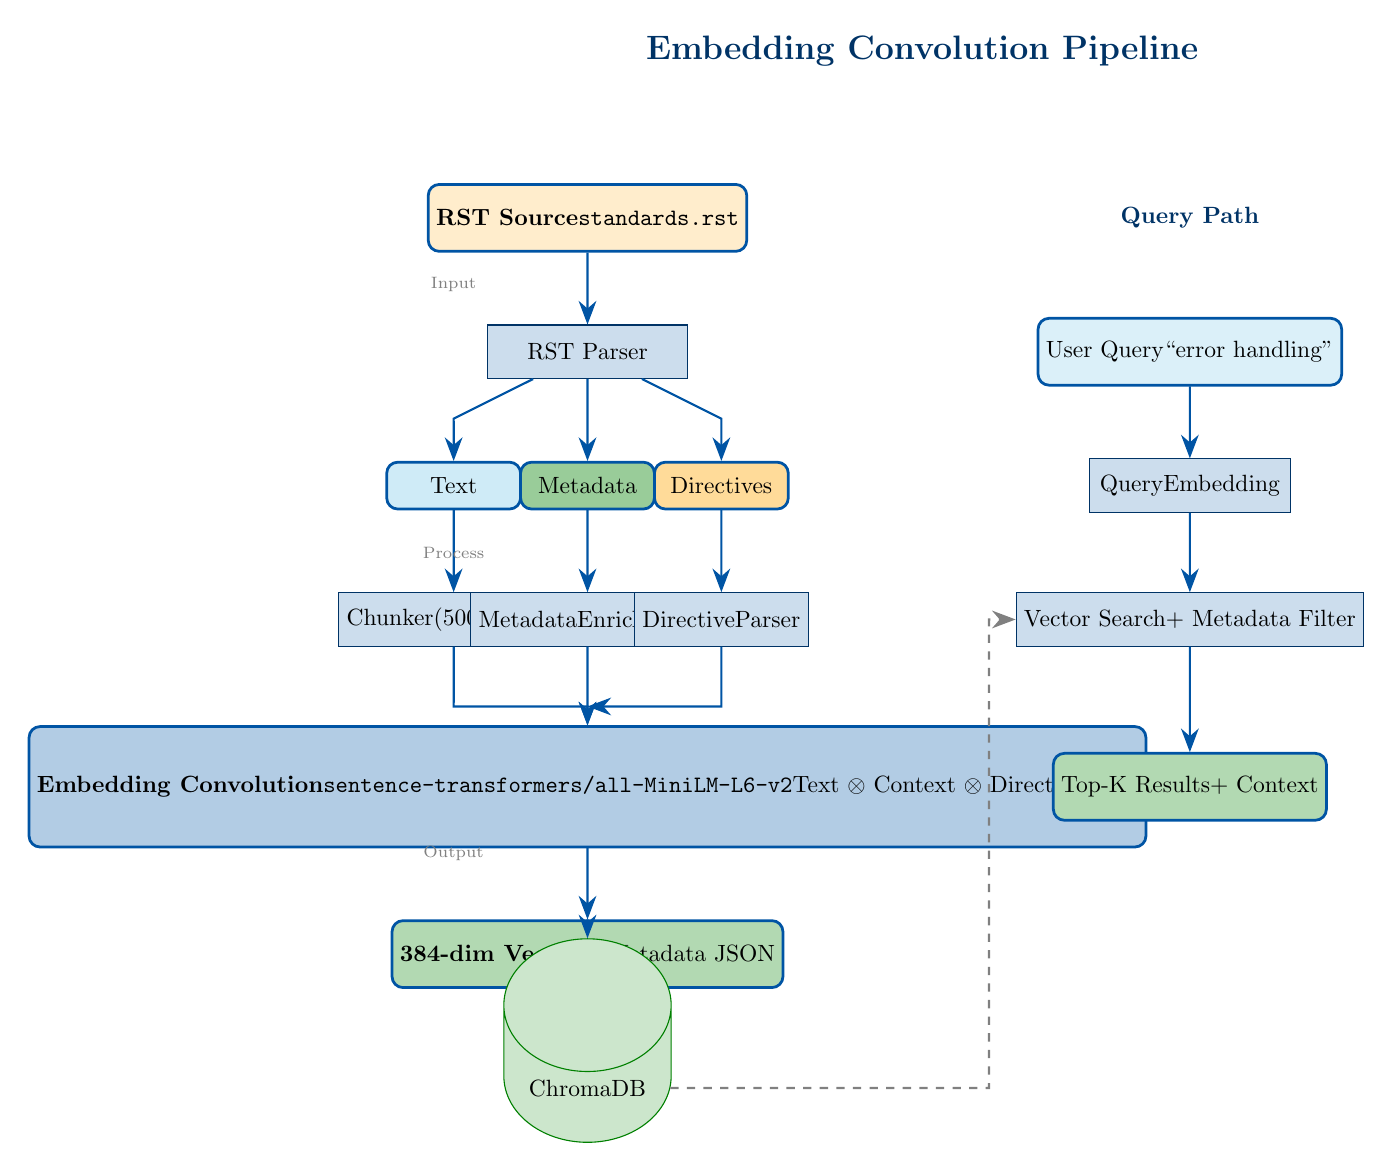
\begin{tikzpicture}[node distance=0.8cm, scale=0.85, transform shape]

% Title
\node[font=\Large\bfseries, noaadarkblue] at (0, 8) {Embedding Convolution Pipeline};

% Stage 1: Source Document
\node[component, minimum width=4cm, fill=noaaorange!20] (rst) at (-5, 5.5) {
    \textbf{RST Source}\\
    \texttt{standards.rst}
};

% Stage 2: Parser
\node[process, minimum width=3cm] (parser) at (-5, 3.5) {RST Parser};

% Stage 3: Extracted Components
\node[component, minimum width=2cm, minimum height=0.7cm, fill=noaalightblue!40] (text) at (-7, 1.5) {Text};
\node[component, minimum width=2cm, minimum height=0.7cm, fill=noaagreen!40] (meta) at (-5, 1.5) {Metadata};
\node[component, minimum width=2cm, minimum height=0.7cm, fill=noaaorange!40] (dir) at (-3, 1.5) {Directives};

% Stage 4: Processing
\node[process, minimum width=2.5cm] (chunk) at (-7, -0.5) {Chunker\\(500 tokens)};
\node[process, minimum width=2.5cm] (enrich) at (-5, -0.5) {Metadata\\Enrichment};
\node[process, minimum width=2.5cm] (parse) at (-3, -0.5) {Directive\\Parser};

% Stage 5: Convolution
\node[component, minimum width=8cm, minimum height=1.8cm, fill=noaablue!30] (convolve) at (-5, -3) {
    \textbf{Embedding Convolution}\\
    \texttt{sentence-transformers/all-MiniLM-L6-v2}\\
    Text $\otimes$ Context $\otimes$ Directive Tags
};

% Stage 6: Vector Output
\node[component, minimum width=3cm, fill=noaagreen!30] (vector) at (-5, -5.5) {
    \textbf{384-dim Vector}\\
    + Metadata JSON
};

% Stage 7: Storage
\node[data, minimum width=2.5cm] (db) at (-5, -7.5) {ChromaDB};

% Arrows Stage 1-2
\draw[arrow] (rst) -- (parser);

% Arrows Stage 2-3
\draw[arrow] (parser) -- (-7, 2.5) -- (text);
\draw[arrow] (parser) -- (meta);
\draw[arrow] (parser) -- (-3, 2.5) -- (dir);

% Arrows Stage 3-4
\draw[arrow] (text) -- (chunk);
\draw[arrow] (meta) -- (enrich);
\draw[arrow] (dir) -- (parse);

% Arrows Stage 4-5
\draw[arrow] (chunk) -- (-7, -1.8) -- (-5, -1.8) -- (convolve);
\draw[arrow] (enrich) -- (convolve);
\draw[arrow] (parse) -- (-3, -1.8) -- (-5, -1.8);

% Arrows Stage 5-6-7
\draw[arrow] (convolve) -- (vector);
\draw[arrow] (vector) -- (db);

% Right side: Query Path
\node[font=\bfseries, noaadarkblue] at (4, 5.5) {Query Path};

\node[component, minimum width=3.5cm, fill=noaalightblue!30] (query) at (4, 3.5) {
    User Query\\
    ``error handling''
};

\node[process, minimum width=3cm] (qembed) at (4, 1.5) {Query\\Embedding};

\node[process, minimum width=3cm] (search) at (4, -0.5) {Vector Search\\+ Metadata Filter};

\node[component, minimum width=3.5cm, fill=noaagreen!30] (results) at (4, -3) {
    Top-K Results\\
    + Context
};

% Query arrows
\draw[arrow] (query) -- (qembed);
\draw[arrow] (qembed) -- (search);
\draw[dashedarrow] (db) -- (1, -7.5) -- (1, -0.5) -- (search);
\draw[arrow] (search) -- (results);

% Labels
\node[font=\scriptsize, noaagray] at (-7, 4.5) {Input};
\node[font=\scriptsize, noaagray] at (-7, 0.5) {Process};
\node[font=\scriptsize, noaagray] at (-7, -4) {Output};

\end{tikzpicture}
\caption{Embedding Convolution: How RST Directives Become Searchable Vectors}
\label{fig:pipeline}
\end{figure}

\newpage
%=============================================================================
\section{False Positive Reduction Results}
%=============================================================================

\begin{figure}[H]
\centering
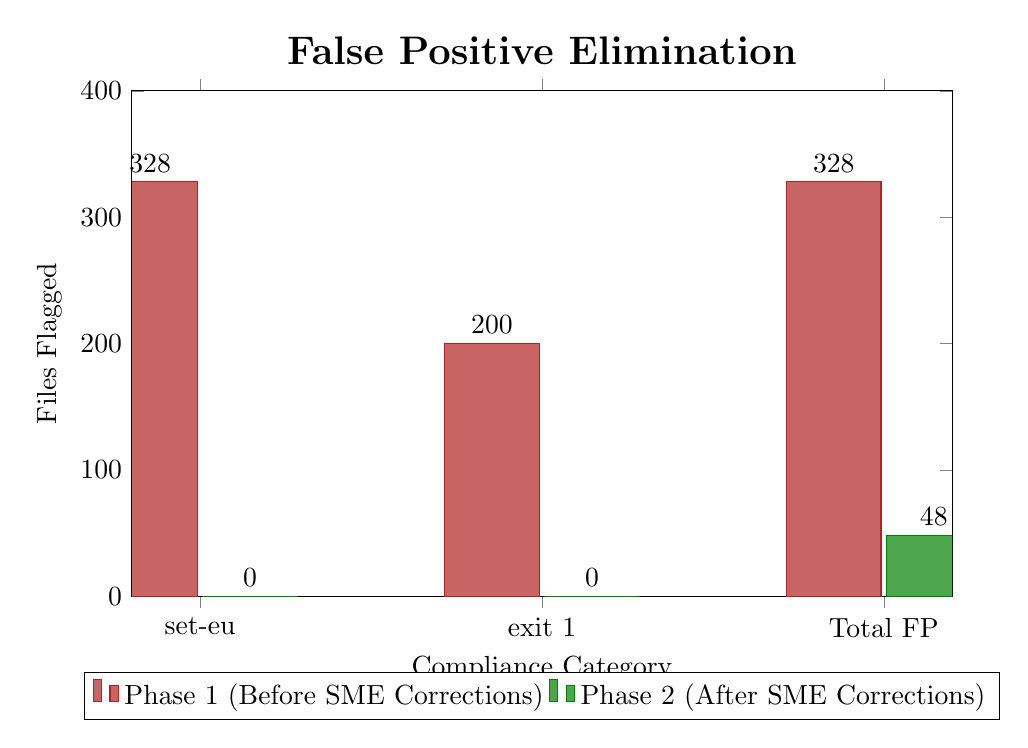
\begin{tikzpicture}
\begin{axis}[
    ybar,
    width=12cm,
    height=8cm,
    bar width=1.2cm,
    ylabel={Files Flagged},
    xlabel={Compliance Category},
    ymin=0,
    ymax=400,
    symbolic x coords={set-eu, exit 1, Total FP},
    xtick=data,
    nodes near coords,
    nodes near coords align={vertical},
    legend style={at={(0.5,-0.15)}, anchor=north, legend columns=2},
    title={\textbf{False Positive Elimination}},
    title style={font=\Large},
]
% Phase 1 (Before)
\addplot[fill=noaared!70, draw=noaared] coordinates {
    (set-eu, 328)
    (exit 1, 200)
    (Total FP, 328)
};
% Phase 2 (After)
\addplot[fill=noaagreen!70, draw=noaagreen] coordinates {
    (set-eu, 0)
    (exit 1, 0)
    (Total FP, 48)
};
\legend{Phase 1 (Before SME Corrections), Phase 2 (After SME Corrections)}
\end{axis}
\end{tikzpicture}
\caption{85\% Reduction in False Positives Through Semantic Annotations}
\label{fig:fp-reduction}
\end{figure}

%=============================================================================
\section{MCP Directive Distribution}
%=============================================================================

\begin{figure}[H]
\centering
\begin{tikzpicture}
\begin{axis}[
    xbar,
    width=12cm,
    height=10cm,
    bar width=0.6cm,
    xlabel={Number of Directives},
    ylabel={Directive Type},
    xmin=0,
    xmax=20,
    symbolic y coords={
        llm\_validation\_prompt,
        context\_types,
        utility,
        ai\_guidance\_rule,
        sme\_correction,
        anti\_pattern,
        correct\_pattern,
        intent,
        compliance
    },
    ytick=data,
    nodes near coords,
    nodes near coords align={horizontal},
    title={\textbf{63 MCP Directives by Type}},
    title style={font=\Large},
]
\addplot[fill=noaablue!70, draw=noaablue] coordinates {
    (15, compliance)
    (12, intent)
    (10, correct\_pattern)
    (8, anti\_pattern)
    (6, sme\_correction)
    (5, ai\_guidance\_rule)
    (3, utility)
    (2, context\_types)
    (2, llm\_validation\_prompt)
};
\end{axis}
\end{tikzpicture}
\caption{Distribution of MCP Directive Types in standards.rst}
\label{fig:directives}
\end{figure}

\newpage
%=============================================================================
\section{EE2 Category Coverage}
%=============================================================================

\begin{figure}[H]
\centering

\begin{tikzpicture}
\pie[
    text=legend,
    radius=4,
    color={noaablue!70, noaagreen!70, noaaorange!70, noaared!50, 
           noaalightblue!70, noaagray!50, noaablue!30, noaagreen!30},
    explode={0.1, 0, 0, 0, 0, 0, 0, 0}
]{
    24/Error Handling (15),
    19/Environment Variables (12),
    16/File Naming (10),
    13/Production Utilities (8),
    10/Workflow Structure (6),
    8/Code Standards (5),
    6/Directory Structure (4),
    5/Logging (3)
}
\node[font=\Large\bfseries] at (0, 5) {EE2 Compliance Categories};
\end{tikzpicture}
\caption{Distribution of Annotations Across EE2 Compliance Categories}
\label{fig:categories}
\end{figure}

%=============================================================================
\section{System Component Diagram}
%=============================================================================

\begin{figure}[H]
\centering
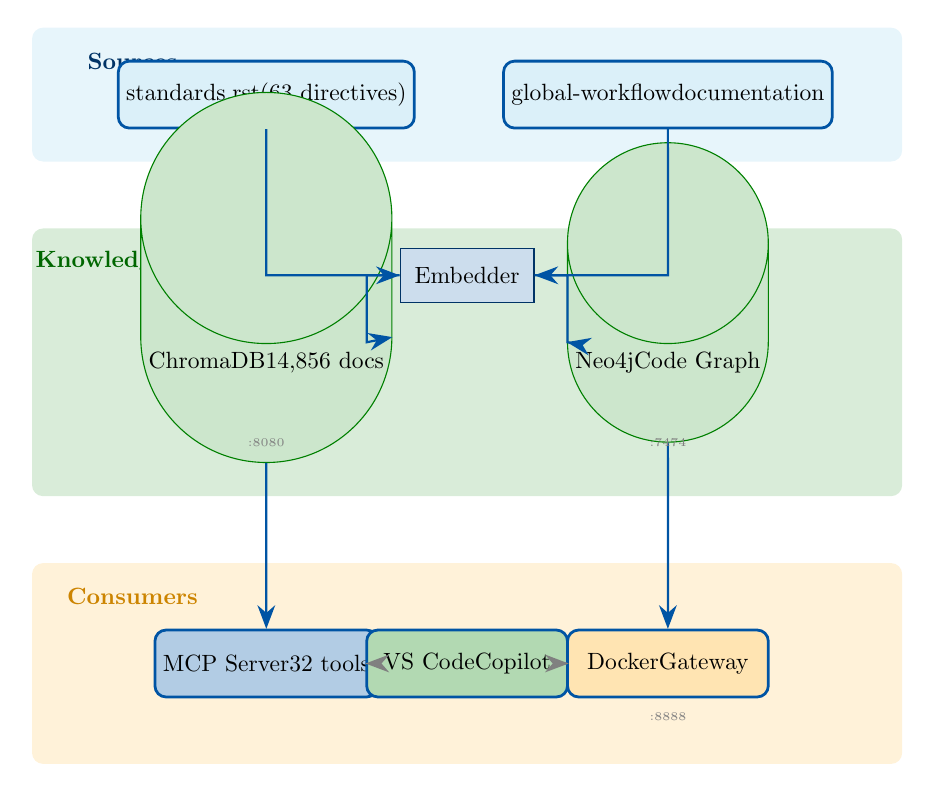
\begin{tikzpicture}[node distance=1.5cm, scale=0.85, transform shape]

% Background boxes
\begin{scope}[on background layer]
    \fill[noaalightblue!20, rounded corners] (-6.5, 4.5) rectangle (6.5, 6.5);
    \fill[noaagreen!15, rounded corners] (-6.5, -0.5) rectangle (6.5, 3.5);
    \fill[noaaorange!15, rounded corners] (-6.5, -4.5) rectangle (6.5, -1.5);
\end{scope}

% Labels
\node[font=\bfseries, noaadarkblue] at (-5, 6) {Sources};
\node[font=\bfseries, noaagreen!80!black] at (-5, 3) {Knowledge Base};
\node[font=\bfseries, noaaorange!80!black] at (-5, -2) {Consumers};

% Source layer
\node[component, minimum width=4cm] (standards) at (-3, 5.5) {standards.rst\\(63 directives)};
\node[component, minimum width=4cm] (gwdocs) at (3, 5.5) {global-workflow\\documentation};

% Knowledge layer
\node[data, minimum width=2.5cm] (chromadb) at (-3, 1.5) {ChromaDB\\14,856 docs};
\node[data, minimum width=2.5cm] (neo4j) at (3, 1.5) {Neo4j\\Code Graph};
\node[process, minimum width=2cm] (embedder) at (0, 2.8) {Embedder};

% Consumer layer
\node[component, minimum width=3cm, fill=noaablue!30] (mcp) at (-3, -3) {MCP Server\\32 tools};
\node[component, minimum width=3cm, fill=noaagreen!30] (vscode) at (0, -3) {VS Code\\Copilot};
\node[component, minimum width=3cm, fill=noaaorange!30] (gateway) at (3, -3) {Docker\\Gateway};

% Arrows
\draw[arrow] (standards) -- (-3, 4) -- (-3, 2.8) -- (embedder);
\draw[arrow] (gwdocs) -- (3, 4) -- (3, 2.8) -- (embedder);
\draw[arrow] (embedder) -- (-1.5, 2.8) -- (-1.5, 1.8) -- (chromadb);
\draw[arrow] (embedder) -- (1.5, 2.8) -- (1.5, 1.8) -- (neo4j);

\draw[arrow] (chromadb) -- (-3, -1.8) -- (mcp);
\draw[arrow] (neo4j) -- (3, -1.8) -- (gateway);
\draw[dashedarrow] (mcp) -- (vscode);
\draw[dashedarrow] (gateway) -- (vscode);

% Port annotations
\node[font=\tiny, noaagray] at (-3, 0.3) {:8080};
\node[font=\tiny, noaagray] at (3, 0.3) {:7474};
\node[font=\tiny, noaagray] at (3, -3.8) {:8888};

\end{tikzpicture}
\caption{MCP-RAG System Components and Data Flow}
\label{fig:components}
\end{figure}

\newpage
%=============================================================================
\section{Update Workflow}
%=============================================================================

\begin{figure}[H]
\centering
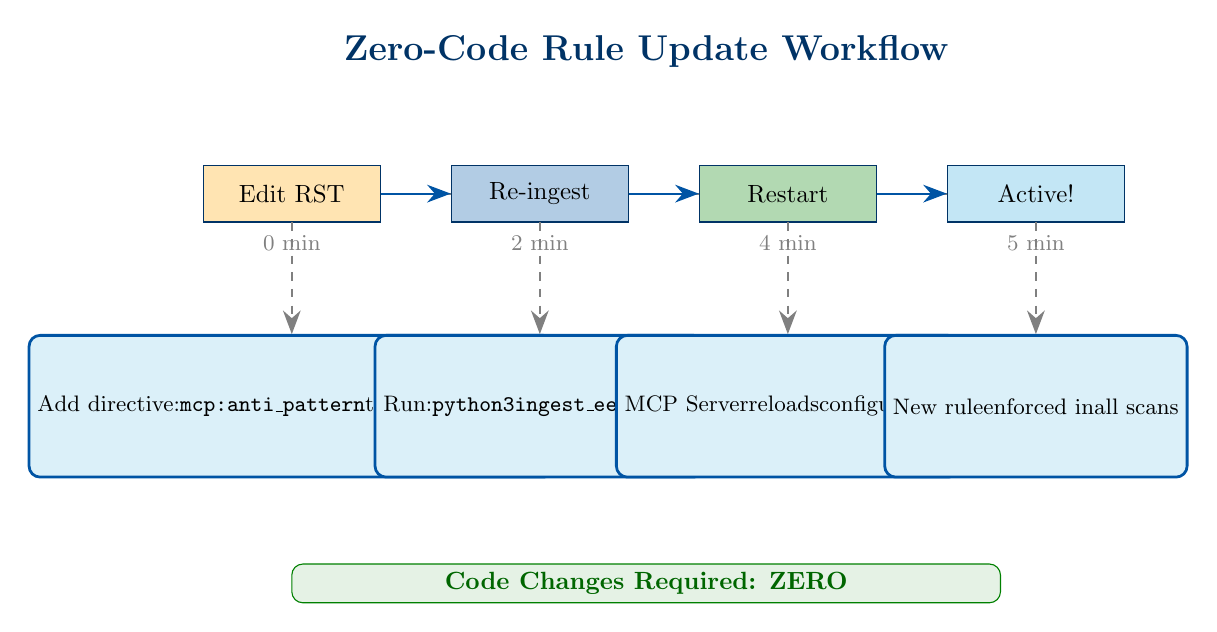
\begin{tikzpicture}[node distance=1.2cm, scale=0.9, transform shape]

% Title
\node[font=\Large\bfseries, noaadarkblue] at (0, 7) {Zero-Code Rule Update Workflow};

% Timeline
\draw[thick, noaagray] (-6, 5) -- (6, 5);

% Steps
\node[process, minimum width=2.5cm, fill=noaaorange!30] (step1) at (-5, 5) {Edit RST};
\node[process, minimum width=2.5cm, fill=noaablue!30] (step2) at (-1.5, 5) {Re-ingest};
\node[process, minimum width=2.5cm, fill=noaagreen!30] (step3) at (2, 5) {Restart};
\node[process, minimum width=2.5cm, fill=noaalightblue!50] (step4) at (5.5, 5) {Active!};

% Time labels
\node[font=\small, noaagray] at (-5, 4.3) {0 min};
\node[font=\small, noaagray] at (-1.5, 4.3) {2 min};
\node[font=\small, noaagray] at (2, 4.3) {4 min};
\node[font=\small, noaagray] at (5.5, 4.3) {5 min};

% Details
\node[component, minimum width=3.5cm, minimum height=2cm, font=\small] (d1) at (-5, 2) {
    Add directive:\\
    \texttt{mcp:anti\_pattern}\\
    to \texttt{standards.rst}
};
\node[component, minimum width=3.5cm, minimum height=2cm, font=\small] (d2) at (-1.5, 2) {
    Run:\\
    \texttt{python3}\\
    \texttt{ingest\_ee2\_v7.py}
};
\node[component, minimum width=3.5cm, minimum height=2cm, font=\small] (d3) at (2, 2) {
    MCP Server\\
    reloads\\
    configuration
};
\node[component, minimum width=3.5cm, minimum height=2cm, font=\small] (d4) at (5.5, 2) {
    New rule\\
    enforced in\\
    all scans
};

% Arrows
\draw[arrow] (step1) -- (step2);
\draw[arrow] (step2) -- (step3);
\draw[arrow] (step3) -- (step4);

\draw[dashedarrow] (step1) -- (d1);
\draw[dashedarrow] (step2) -- (d2);
\draw[dashedarrow] (step3) -- (d3);
\draw[dashedarrow] (step4) -- (d4);

% Bottom note
\node[draw=noaagreen, fill=noaagreen!10, rounded corners, minimum width=10cm, 
      font=\bfseries, text=noaagreen!80!black] at (0, -0.5) {
    Code Changes Required: ZERO
};

\end{tikzpicture}
\caption{5-Minute Update Workflow with Zero Code Changes}
\label{fig:workflow}
\end{figure}

%=============================================================================
\section{Before/After Comparison}
%=============================================================================

\begin{figure}[H]
\centering
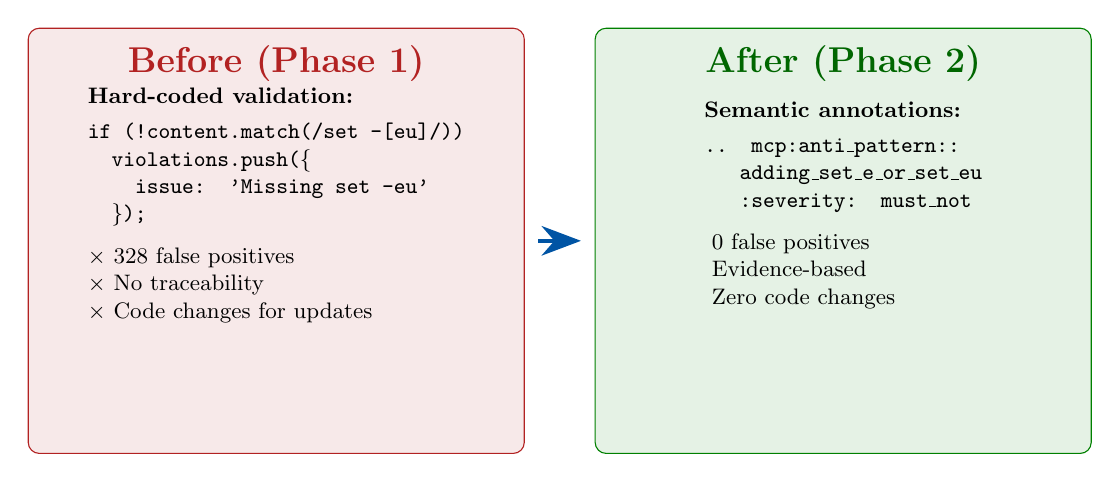
\begin{tikzpicture}[scale=0.9, transform shape]

% Before box
\node[draw=noaared, fill=noaared!10, rounded corners, minimum width=7cm, minimum height=6cm] 
    (before) at (-4, 0) {};
\node[font=\Large\bfseries, noaared] at (-4, 2.5) {Before (Phase 1)};
\node[align=left, font=\small] at (-4, 0.5) {
    \textbf{Hard-coded validation:}\\[3pt]
    \texttt{if (!content.match(/set -[eu]/))}\\
    \texttt{\ \ violations.push(\{}\\
    \texttt{\ \ \ \ issue: 'Missing set -eu'}\\
    \texttt{\ \ \});}\\[6pt]
    $\times$ 328 false positives\\
    $\times$ No traceability\\
    $\times$ Code changes for updates
};

% After box
\node[draw=noaagreen, fill=noaagreen!10, rounded corners, minimum width=7cm, minimum height=6cm] 
    (after) at (4, 0) {};
\node[font=\Large\bfseries, noaagreen!80!black] at (4, 2.5) {After (Phase 2)};
\node[align=left, font=\small] at (4, 0.5) {
    \textbf{Semantic annotations:}\\[3pt]
    \texttt{.. mcp:anti\_pattern::}\\
    \texttt{\ \ \ adding\_set\_e\_or\_set\_eu}\\
    \texttt{\ \ \ :severity: must\_not}\\[6pt]
    \checkmark\ 0 false positives\\
    \checkmark\ Evidence-based\\
    \checkmark\ Zero code changes
};

% Arrow
\draw[-{Stealth[length=5mm]}, ultra thick, noaablue] (-0.3, 0) -- (0.3, 0);

\end{tikzpicture}
\caption{Transformation from Hard-Coded to Semantic Validation}
\label{fig:comparison}
\end{figure}

\newpage
%=============================================================================
\section{Summary Table}
%=============================================================================

\begin{table}[H]
\centering
\caption{MCP Semantic Annotations System Metrics}
\label{tab:metrics}
\begin{tabular}{@{}lrl@{}}
\toprule
\textbf{Metric} & \textbf{Value} & \textbf{Notes} \\
\midrule
\multicolumn{3}{l}{\textit{Knowledge Base}} \\
ChromaDB Collections & 12 & v7.0.0 architecture \\
Total Documents & 14,856 & Across all collections \\
EE2 Chunks & 94 & standards.rst content \\
MCP Directives & 63 & Inline in standards.rst \\
Embedding Dimensions & 384 & MiniLM-L6-v2 model \\
\midrule
\multicolumn{3}{l}{\textit{Compliance Impact}} \\
False Positive Reduction & 85\% & 328 → 48 violations \\
set -eu FP Eliminated & 100\% & 328 → 0 files \\
exit 1 FP Eliminated & 100\% & 200 → 0 files \\
\midrule
\multicolumn{3}{l}{\textit{Operational}} \\
MCP Tools Available & 32 & 7 tool modules \\
Rule Update Time & 5 min & Zero code changes \\
Config Load Time & <100ms & At server startup \\
Scan Speed & 18ms/file & No runtime DB queries \\
\bottomrule
\end{tabular}
\end{table}

%=============================================================================
\section{Appendix: Compiling This Document}
%=============================================================================

To compile this document:

\begin{verbatim}
# Local compilation
pdflatex mcp_semantic_annotations_figures.tex
pdflatex mcp_semantic_annotations_figures.tex  # Run twice for ToC

# Or use latexmk
latexmk -pdf mcp_semantic_annotations_figures.tex

# Required packages:
# - tikz, pgfplots
# - booktabs, float
\end{verbatim}

For Overleaf: Upload this file directly and compile.

\vfill
\noindent\rule{\textwidth}{0.5pt}\\
\small{NOAA/EMC Environmental Information Branch | December 2025 | v2.0.0}

\end{document}
